\documentclass[12pt]{beamer}
\usepackage{fontspec}
\usepackage{color}
\usepackage{minted}

%% These fonts are non-free.
%% Comment out the lines if you don't have them.
\setmainfont{Equity Text A}
\setsansfont{Concourse T3}
\setmonofont{Triplicate T4}

\definecolor{bgcolor}{RGB}{20,25,28}
\setbeamercolor{background canvas}{bg=bgcolor}
\setbeamercolor{normal text}{fg=white}
\setbeamercolor{itemize item}{fg=white}
\setbeamertemplate{itemize items}[circle]
\usemintedstyle{monokai}

\renewcommand{\theFancyVerbLine}{\color{darkgray}\large \oldstylenums{\arabic{FancyVerbLine}}}
\newcommand{\toptitle}[1]{
  {\huge #1} \\
  \vspace{0.2cm}
}
\renewcommand{\subtitle}[1]{
  {\large #1} \\
  \vspace{0.2cm}
}

\newcommand*{\shifttext}[2]{%
  \settowidth{\@tempdima}{#2}%
  \makebox[\@tempdima]{\hspace*{#1}#2}%
}

\begin{document}
\begin{frame}
  \begin{center}
    
\includegraphics[height=4cm]{avatar.png}\\
    \vspace{0.2cm}
    {\Large Nicolas Hafner} \\
    \vspace{0.2cm}
    {\Huge @Shinmera} \\
    \vspace{0.2cm}
    \url{https://everything.shinmera.com}
  \end{center}
\end{frame}

\begin{frame}
  \toptitle{Radiance - A Web Framework Environment for Common Lisp}
\end{frame}

%% Standard frameworks are oriented around single-purpose sites
\begin{frame}
  \toptitle{Usual Framework Focus}
  \begin{itemize}
    \item Single application
    \item Tightly integrated
    \item Convenience through large toolsets
      \pause
    \item Often force libraries on you
      \pause
    \item Problematic to host multiple applications
  \end{itemize}
\end{frame}

%% Radiance is an application-universe
\begin{frame}
  \toptitle{Radiance's Goals}
  \begin{itemize}
    \item Many applications simultaneously
    \item Shared resources
    \item Exchangeable parts
    \item Only use what you want
      \pause
    \item Fully specified
  \end{itemize}
\end{frame}

\begin{frame}
  \toptitle{A Tiny Example}
  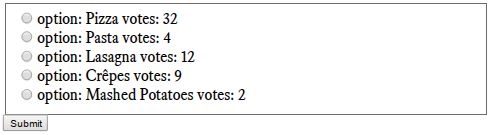
\includegraphics[height=3cm]{voter.png}
\end{frame}

%% Writing an application is very easy
\begin{frame}[fragile]
  \begin{minted}{common-lisp}
(in-package #:rad-user)
(db:create 'vote '((option (:varchar 32))
                   (votes :integer)))

(define-page display #@"/" ()
  (r-forms:choose 
   #@"/api/vote" "id"
   (dm:get 'vote (db:query :all))))

(define-api vote (id) ()
  (with-model-save model ('vote (:= '_id id))
      (votes)
    (incf votes))
  (redirect #@"/")
  (api-output "Vote registered."))
  \end{minted}
\end{frame}

%% It also offers a complete segregation through interfaces
\begin{frame}[fragile]
  \begin{minted}{common-lisp}
(define-interface (database db)
  (defun create (collection structure 
                 &key indices if-exists))
  (defmacro query (query-form))
  ...)

(define-interface (data-model dm)
  (defun get (collection query 
              &key (skip 0) (amount 0) sort))
  ...)
  \end{minted}
\end{frame}

%% and the implementors thereof
\begin{frame}[fragile]
  \begin{minted}{common-lisp}
(define-module #:my-database
  (:use #:cl)
  (:implements #:database))
(in-package #:my-database)

(defun db:create (database db
                  &key indices if-exists)
  ...)

(defmacro db:query (query-form)
  ...)

...
  \end{minted}
\end{frame}

%% Architecture
\begin{frame}
\vspace{0.5cm}
\toptitle{What Radiance Offers}
\begin{\large}
\begin{columns}[T]
\begin{column}[T]{5cm}
Modules \\
Interfaces \\
Request handling \\
URIs \\
URI Patterns \\
Resources \\
Bidirectional Routing \\
Dispatching \\
\pause
Banning \\
Rate limiting \\
Administration interface \\
Cache handling \\
Authentication \\
\end{column}
\begin{column}[T]{5cm}
Sessions \\
User storage \\
User profiles \\
Logging \\
Database interaction \\
DB abstractions \\
Templating \\
Error handling \\
\pause
Chatlog \\
Blog software \\
File hosting \\
Imageboard \\
Database introspection \\
Keyword reviews \\
User management \\
Paste service \\
\end{column}
\end{columns}
\end{large}
\end{frame}

%% Link / Install
\begin{frame}[fragile]
  \begin{center}
    \includegraphics[height=3cm]{radiance-logo.png} \\
    {\bfseries \url{https://github.com/Shirakumo/radiance}} \\
    \vspace{0.3cm}
    \begin{minted}{common-lisp}
(ql-dist:install-dist 
 "http://dist.tymoon.eu/shirakumo.txt")
(ql:quickload :radiance)
(radiance:startup)
    \end{minted}
  \end{center}
\end{frame}

\end{document}

%%% Local Variables:
%%% mode: latex
%%% TeX-command-extra-options: "-shell-escape"
%%% TeX-master: t
%%% TeX-engine: luatex
%%% End:
